%& --translate-file=cp1250pl
\documentclass[11pt,a4paper]{article}
\usepackage[left=3.5cm, right=4cm, bottom=6.65cm, top=5cm]{geometry}

\usepackage{amssymb}
\usepackage{amsmath}
\usepackage{setspace}
\usepackage{setspace}
\usepackage{array}
\usepackage{longtable}
\usepackage{tabularx}
\usepackage{multicol}
\usepackage{graphics}
\usepackage{graphicx}
\usepackage{times}
\usepackage{algorithmic}
\usepackage{algorithm}
\usepackage{array,multirow,graphicx}

%=========================================================================%
%============================== Definitions ==============================%
%=========================================================================%

\makeatletter

\bibliographystyle{plain}
\newtheorem{theorem}{Theorem}
\newtheorem{proof}{Proof}
\newtheorem{lemma}{Lemma}
\newtheorem{property}{Property}
\newtheorem{corollary}{Corollary}
\newtheorem{procedure}{Procedure}


\def\tablename{Table}
\def\figurename{Fig.}

\pagestyle{empty}

\renewcommand{\theenumi}{\roman{enumi})}
%\def\secsize{18pt}

\renewcommand{\thefootnote}{\fnsymbol{footnote}}


\newcommand\sectionsize{\fontsize{11}{12}\selectfont}
\newcommand\subsectionsize{\fontsize{9}{12}\selectfont}
\newcommand\refefencesize{\fontsize{10}{12}\selectfont}

\newcommand{\Booktitle}[1]{
\begin{flushleft}
\fontsize{10pt}{0pt}\selectfont \fontfamily{\sfdefault}\noindent \vspace{1pt}  \textbf{#1} \fontfamily{\familydefault} \\[12pt]
\end{flushleft}}

\newcommand{\Keywords}[1]{
\begin{flushright}
{\fontsize{9pt}{0pt}\selectfont \textit{Keywords: #1}} \\[13pt]
\end{flushright}}

\newcommand{\Title}[1]{
{\fontsize{13pt}{15pt}\selectfont
\begin{center}
 \textbf{#1} \\[36pt]
\end{center}}}

\newcommand{\Abstract}[1]{\setlength{\parindent}{5mm}
\parbox{13cm}{ \fontsize{9pt}{12pt}\selectfont \setlength{\parindent}{5mm} #1}}


%\renewcommand\caption{\fontsize{9}{1}\selectfont #1}

\newcommand{\captionfonts}{\fontsize{9}{1}\selectfont}

\setlength\abovecaptionskip{0pt}
\setlength\belowcaptionskip{0pt}
\newlength\abovetableskip
\newlength\belowtableskip
\newlength\abovefigureskip
\newlength\belowfigureskip
\setlength\abovetableskip{0pt}
%
\setlength\belowtableskip{6pt}
%
\setlength\abovefigureskip{6pt}
%
\setlength\belowfigureskip{0pt}

\long\def\@makecaption#1#2{%
  \vskip\abovecaptionskip
  \sbox\@tempboxa{{\captionfonts #1. #2 }}%
  \ifdim \wd\@tempboxa >\hsize
    {\captionfonts #1. #2\par}
  \else
    \hbox to\hsize{\hfil\box\@tempboxa\hfil}%
  \fi
  \vskip\belowcaptionskip}

\renewenvironment{table}{%
   %\let \@makecaption \@maketablecaption
   \setlength{\abovecaptionskip}{\abovetableskip}
   \setlength{\belowcaptionskip}{\belowtableskip}
   \@float{table}}%
   {\end@float}

\renewenvironment{figure}{%
  \setlength{\abovecaptionskip}{\abovefigureskip}
  \setlength{\belowcaptionskip}{\belowfigureskip} \vspace{0pt}
  \@float{figure}}%
  {\end@float}


\renewcommand\section{\@startsection {section}{1}{0cm}%
                                   {24pt}%
                                   {15pt}%
                                   {\centering\normalfont\sectionsize}}

\renewcommand\subsection{\@startsection {subsection}{2}{0cm}%
                                   {9pt}%
                                   {9pt}%
                                   {\centering\normalfont\subsectionsize}}

\renewcommand{\@seccntformat}[1]{\csname the#1\endcsname.\quad }

\def\refname{{\sectionsize REFERENCES}}
\def\refsize{\refefencesize}


%=========================================================================%
%========================== Author(s) & Title ============================%
%=========================================================================%

\begin{document}
%
\Booktitle{Computer Systems Engineering 2007 (co tu wpisac?)}
%
\Keywords{american sign language, images recognition, machine learning}
%

\noindent Mi\l osz BIA\L CZAK\footnote{\noindent Wroc\l aw University of Science and Technology, Poland\label{pwr1}} \\
%
\noindent Martyna \L AGO\.ZNA\textsuperscript{\ref{pwr1}} \\[7pt]
%
\Title{AMERICAN SIGN LANGUAGE RECOGNITION}


%=========================================================================%
%============================== Abstract =================================%
%=========================================================================%

\Abstract{
	What if the fast development of computer science, especially machine learning could help disabled people? In fact, it can and this is the topic to which the research described in this paper has been devoted. Deaf-mute people are the part of our society and it would be a great convenience both for them and speaking people which would allow for a better communication using technology. In this paper, the results of research concerning recognition of sign language has been shared. The research includes experimenting with the images transformations and usage of different learning and features detecting algorithms to obtain the best quality of signs recognition. In addition the part of this work has been also the impact of background and different hands rotation.
}


%=========================================================================%
%=========================== INTRODUCTION ================================%
%=========================================================================%

\section{INTRODUCTION}

	Nowadays, using technology to solve medical issues is becoming a common practice[]. Constant and fast development of science and growing popularity of machine learning allow for creating technologically advanced appliances and complex algorithms which are aimed at helping people. Sign language recognition is an interesting and significant issue strictly connected with both machine learning and medical technology. Deaf-mute people pose X\% of the whole society[]. In the past there were no technical possibilities to facilitate their lives and communication ways. Now it is still challenging but possible so we attempted to solve this issue. 

	In this work we decided to experiment with different features extraction and learning algorithms and pay particular attention on image processing. Moreover the scope of this work includes also checking the impact of background and hands rotations on received accuracy based on usage 2 completely different data sets.
	
	Our approach to this problem at the current stage is based on recognition of single letters from American sign language alphabet. One of the crucial assumptions of this work is recognition of images taken with average-quality camera because the algorithm which has been implemented should be available for everyone for example by a build-in camera in mobile phone or computer.
	
	
	
	
	

	
%=========================================================================%
%========================= PROBLEM FORMULATION ===========================%
%=========================================================================%

\section{PROBLEM FORMULATION}

	The objective of this work is to create an algorithm which recognizes static gestures of single letters from American sign language alphabet with the highest possible accuracy. The algorithm should be given an image in .jpg format on input and the result should be returned as recognized letter on string type. To implement the algorithm, it is necessary to consider the problems as follows:
	
* finding crucial features and point on the picture

* emphasizing of hand features
	
* finding satisfying way of learning the algorithm.








%=========================================================================%
%============================= ALGORITHMS ================================%
%=========================================================================%

\section{ALGORITHMS}

	In this section, the algorithms used in this work are being
	\begin{figure}[H]
		\centering
		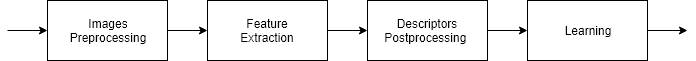
\includegraphics[width=0.9\textwidth]{Algorithm.png}
		\caption{Preprocessing data flow}
		\label{fig:Algorithm}
	\end{figure} 

\subsection{Preprocessing}
	
	To prepare the set of images and improve received results Gaussian blur and anisotropic filtering has been used. Gaussian blur is a method of modification the image with Gaussian function. It is commonly used to reduce image noise and reduce details. Anisotropic filtering is a technique of enhancing the image quality... nie wiem co tu napsiac o tym, trzeba poczukac odwolania do czegos madrego o tym. In our work we used Gaussian blur to avoid recognition of unimportant and excess points which potentially could be found by the algorithm. At the same time, to sharpen the shape of hand and to not lose the main shape of the gesture anisotropic filtering has been applied.
	
	
	\begin{figure}[H]
		\centering
		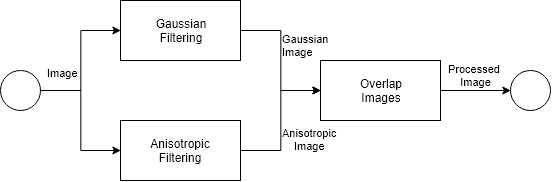
\includegraphics[width=0.9\textwidth]{Preprocessing.png}
		\caption{Preprocessing data flow}
		\label{fig:Preprocessing}
	\end{figure}

\subsection{Features extraction}

In our research we use three different feature extractors from \textit{ski-image} library, to find with one will be bather to our purposes.

\begin{itemize}
	\item \textit{CENSURE}\cite{CENSURE} - The new on kind of extractor, witch biggest feature is fast compute time, what make it a good candidate project purposes. Unfortunate CENSURE find only the key point on the picture and to take descriptors from them in need to be supported other descriptors extractor, in our implementation that was BRIEF.
	
	\item \textit{BRIEF}\cite{BRIEF} - Binary Robust Independent Elementary Features is an efficient feature point descriptor. The standard feature extraction method with. It is highly discriminative even when using relatively few bits and is computed using simple intensity difference tests. That extractor have also one difficulty, it's not good working with rotations. 
	
	\item \textit{ORB}\cite{ORB} - Oriented FAST\cite{FAST} and rotated BRIEF feature detector and binary descriptor extractor. It is based on FAST key point detector and modified BRIEF to good work with rotations. It's also fast compute so it is preferred for real-time applications, that why we also interested in it.
\end{itemize}

\subsection{Postprocessing}

After features extraction and before classifier learning, extracted data need some improvement, to be more reliable. To do that we use two steps normalization.

\begin{itemize}
	\item \textit{Normalize} \cite{PREPROCESSING}  - rescales the vector for each sample to have unit norm, independently of the distribution of the samples.
	
	\item \textit{Standard Scaler} \cite{PREPROCESSING}  - removes the mean and scales the data to unit variance. However, the outliers have an influence when computing the empirical mean and standard deviation which shrink the range of the feature values. Standard Scaler unfortunately cannot guarantee balanced feature scales in the presence of outliers.
\end{itemize}

\begin{figure}[H]
	\centering
	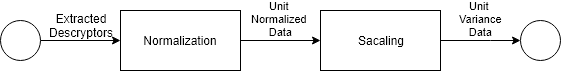
\includegraphics[width=0.9\textwidth]{Postprocessing.png}
	\caption{Posteprocessing data flow}
	\label{fig:Posteprocessing}
\end{figure}

\subsection{Learning}

Support Vector Machines (SVMs) are a set of related methods for supervised learning, applicable to both classification and regression problems. A SVM classifiers creates a maximum-margin hyperplane that lies in a transformed input space and splits the example classes, while maximizing the distance to the nearest cleanly split examples. The parameters of the solution hyperplane are derived from a quadratic programming optimization problem\cite{SVM1}.

\begin{itemize}
	\item vector - classifier learned by vector of descriptors from picture with informing what letter is on the picture. That way have a big disadvantaged, because vectors to classifier need to have o the same length, so do big vectors need to be catted, also to short vectors are ignored.
	
	\item points - classifier learned descriptor after descriptor from picture, with information to what letter is connected. That way of learning make algorithm independent to data vector length.
	
	\item combined - using both points and vector classifiers, and learn from they outputs, with one is correct.
\end{itemize}

%=========================================================================%
%================================ EXPERIMENTS ============================%
%=========================================================================%

\section{EXPERIMENT}

\subsection{Data sets}
	In this experiment two different data sets has been used. The first one has been downloaded from the website of Silesian University of Technology[czy tu powinien byc odnosnik do tego zbioru?]. It consists of 899 images of gestures from American aplhabet form A to Y excluding J. Letters 'Z' and 'J' are moving gestures and it is impossible to show them on single picture. This data set contains images with uncontrolled background and lightning conditions, different angle of hand rotations form observer perspective and different resolution. Images are oriented both vertically and horizontally.
	
	The second data set used in the experiment is a self-made set of images which has been created in possibly similar lightning condition. On each image only hands at uniform, plain background has been shown. Each image has exactly the same, high resolution and all of them are oriented horizontally. The set contains images of gestures of all American sign alphabet also with 'J' and 'Z' excluded.


%=========================================================================%
%======================== RESULTS OF EXPERIMENTS =========================%
%=========================================================================%

\section{RESULTS}

While the research we adding the new steps to algorithm. And what related to that, by looking on results we in some steps stop using some feature extractors. To understood that behave here is a table with results of research by adding next step to algorithm.


%Wykresy dla danych z Politechniki Śląskiej i dla naszych.
\begin{table}[H]
	\centering
	\begin{tabular}{|c|c|>{\centering}p{1.55cm}|>{\centering}p{1.55cm}|>{\centering}p{1.25cm}|>{\centering}p{1.25cm}|p{2cm}|}
		\cline{3-7}
		\multicolumn{2}{ c| }{}& descriptors & anisotropic filtering & Standard Scaler & Gaussian blur & normalization \\
		\hline
		\multirow{3}{*}{ \rotatebox[origin=c]{90}{\parbox[c]{3.5cm}{\centering ORB} }} & \rotatebox[origin=c]{90}{\parbox[c]{1.5cm}{\centering points}} & 51.72\% & 60.34\% & 91.38\% & 94.84\% & \multicolumn{1}{c|}{ 96.55\% } \\
		\cline{2-7}
		& \rotatebox[origin=c]{90}{\parbox[c]{1.8cm}{\centering combined}} & 13.79\% & 13.79\% & 12.07\% & 13.79\% & \multicolumn{1}{c|}{ 12.07\% } \\
		\cline{2-7}
		& \rotatebox[origin=c]{90}{\parbox[c]{1.5cm}{\centering vector}} & 13.79\% & 13.79\% & 13.79\% & 22.41\% & \multicolumn{1}{c|}{ 25.86\% } \\
		\hline
		\multirow{3}{*}{ \rotatebox[origin=c]{90}{\parbox[c]{3.5cm}{\centering CENSURE} }} & \rotatebox[origin=c]{90}{\parbox[c]{1.5cm}{\centering points}} & 20.69\% & 22.41\% & 15.52\% & 12.07\% & \multicolumn{1}{c|}{ -} \\
		\cline{2-7}
		& \rotatebox[origin=c]{90}{\parbox[c]{1.8cm}{\centering combined}} & 13.79\% & 18.97\% & 15.52\% & 5.17\% & \multicolumn{1}{c|}{ -} \\
		\cline{2-7}
		& \rotatebox[origin=c]{90}{\parbox[c]{1.5cm}{\centering vector}} & 8.61\% & 1.72\% & 0.00\% & 1.72\% & \multicolumn{1}{c|}{ -} \\
		\hline
		\multirow{3}{*}{ \rotatebox[origin=c]{90}{\parbox[c]{3.5cm}{\centering BRIEF} }} & \rotatebox[origin=c]{90}{\parbox[c]{1.5cm}{\centering points}} & 15.52\% & - & - & - & \multicolumn{1}{c|}{ -}\\
		\cline{2-7}
		& \rotatebox[origin=c]{90}{\parbox[c]{1.8cm}{\centering combined}} & 15.52\% & - & - & - & \multicolumn{1}{c|}{ -} \\
		\cline{2-7}
		& \rotatebox[origin=c]{90}{\parbox[c]{1.5cm}{\centering vector}} & 0.00\% & - & - & - & \multicolumn{1}{c|}{ -} \\
		\hline
	\end{tabular}
	\caption{Research results by adding algorithm steps}
	\label{tab:results_by_steps}
\end{table}


Final algorithm was tied on three before mention datasets. Results of that test are below.\\


\begin{table}[H]
	\centering
	\begin{tabular}{|p{5cm}|c|c|c|}
		\cline{1-4}
		\multirow{2}{*}{ datasets } & \multicolumn{3}{ |c| }{ORB} \\
		\cline{2-4}
		& points & combined & vector\\
		\cline{1-4}
		Our set of numbers & 96.55\% & 12.07\% & 25.86\% \\
		\cline{1-4}
		Our set of alphabet & 72.90\% & 3.23\% & 12.26\% \\
		\cline{1-4}
		Set of Silesian University of Technology alphabet & 27.36\% & 3.48\% & 2.49\% \\
		\cline{1-4}
	\end{tabular}
	\caption{Research results by datasets}
	\label{tab:results_by_datasets}
\end{table} 


%=========================================================================%
%============================== CONCLUSION ===============================%
%=========================================================================%

\section{CONCLUSION AND PERSPECTIVES}

After our research we can say the final algorithm we describe is a good base to recognize non-moved gestures on eve background.

%=========================================================================%
%============================== BIBLIOGRAPHY ===============================%
%=========================================================================%

\begin{thebibliography}{99}
\refefencesize \setlength\baselineskip{5pt}
%

\bibitem{CENSURE} 
Adam Schmidt, Marek Kraft, Micha\l $ $ Fularz, Zuzanna Domaga\l a 
\textit{Comparative Assessment of Point Feature Detectors and Descriptors in the Context of Robot Navigation},
Journal of Automation, Mobile Robotics \& Intelligent Systems vol.7 2013.
\bibitem{BRIEF} 
Michael Calonder, Vincent Lepetit, Christoph Strecha, and Pascal Fua, 
\textit{BRIEF: Binary Robust Independent Elementary Features}, 11th European Conference on Computer Vision (ECCV), Heraklion, Crete. LNCS Springer, September 2010.
\bibitem{ORB} 
Ethan Rublee, Vincent Rabaud, Kurt Konolige and Gary Bradski, 
\textit{ORB: an efficient alternative to SIFT or SURF}
 \bibitem{FAST} 
 Edward Rosten and Tom Drummond
\textit{Machine learning for high-speed corner detection},
 2006.
\bibitem{PREPROCESSING} 
Compare the effect of different scalers on data with outliers,
\textit{http://scikit-learn.org/stable/auto\_examples/preprocessing/plot\_all\_scaling.html},
July 2018.
\bibitem{SVM1} Shmilovici Armin \textit{Support Vector Machines} Data Mining and Knowledge Discovery Handbook pp 231-247.


\end{thebibliography}

\listoffigures

\listoftables


\end{document}